
\chapter{Introducción y objetivos}
\noindent El prácticamente ausente ruido de lectura que hace posible la capacidad de medir repetidas veces y de forma no destructiva la carga en cada píxel de un sensor Skipper-CCD, tiene un fuerte impacto a energías por debajo de los $5\,\si{keV}$. En particular, por debajo de los $2\,\si{keV}$ la contribución del ruido de lectura de un CCD convencional a la determinación de estas cantidades puede superar el $30\,\%$. Así es que en este trabajo se propone un estudio sistemático del Factor de Fano a bajas energías, entre $1486\,\si{eV}$ (rayos X del Al) y $677\,\si{eV}$ (rayos X del F).\\
\indent Como parte de este trabajo se propuso el uso de técnicas de análisis de imágenes y procesamiento de datos propias de la física de partículas experimental, lo que llevó al fortalecimiento de conocimientos de estadística y la familiarización con el trabajo científico en un tema de creciente interés. 
Algunas de las metas propuestas en este trabajo fueron:
\begin{enumerate}
    \item Análisis de las mediciones existentes con luz LED para obtener una calibración absoluta del detector a baja ocupancia y a diferentes temperaturas.
    \item Análisis de las mediciones existentes con fluorescencia de rayos X producidos por desexcitación del flúor y aluminio con el objeto de determinar la energía de creación electrón hueco a $677\,\si{eV}$ y $1486\,\si{eV}$ respectivamente. Del mismo análisis se obtendrá también el factor de Fano a dichas energías.
    \item Estudio de la dependencia de las cantidades anteriormente mencionadas con la temperatura en el rango de $123$ a $160\,K$.
    \item Estudio la influencia de otros fuentes de fotones en la construcción de \textit{clusters} y en la determinación del factor de Fano y energía de creación electrón hueco.
    \item De-convolución del efecto que la luz espuria tiene sobre el valor medio de carga y su distribución mediante el desarrollo de simulaciones Montecarlo.
\end{enumerate}
Cabe destacar que la última permitió incrementar la estadística disponible en las imágenes. Esto se debe a que, los cortes de calidad utilizados hasta el momento descartaban eventos que se superponían debido al puente generado por los electrones que induce la luz espuria, transformando así dos o más eventos reales en uno solo. Mitigar este problema generó un mayor aprovechamiento de la estadística disponible y con ello una reducción de las incertezas finales.

\section{Factor de Fano y energía de creación electrón-hueco}
\noindent El factor de Fano es una magnitud que mide la dispersión de una distribución de probabilidad para la carga en un detector. Se define como
\begin{equation*}
    F = \frac{\sigma^{2}}{\mu}
\end{equation*}
donde $\sigma^{2}$ es la varianza de la distribución y $\mu$ es la media o la esperanza. Para el caso particular de una distribución de Poisson, la varianza y la esperanza de la distribución coinciden, de forma que el factor de Fano equivale a $1$.\\
\indent Por otro lado, la energía de creación electrón-hueco $\varepsilon_{\eh}$ es, en valor medio, la energía necesaria para poder producir en un par electrón-hueco en el interior del detector de Silicio.\\
\indent La estimación precisa de ambas magnitudes es de vital importancia en la caracterización de este tipo de detectores, debido que a parámetros como la \textit{eficiencia cuántica} dependen fuertemente de ellos.
%%%%%%%%%%%%%%%%%%%%%%%%%%%%%%%%%%%%%%%%%%%%%%%%%%%%%%%%%%%%%%%%%%

\chapter{Resultados previos}
\noindent En trabajos previos se estudiaron las ventajas de la utilización de la novedosa tecnología \textit{skipper} CCD, para lograr medir con precisión subelectrónica en régimenes de energía donde los sensores CCD convencionales más precisos sólo podrían alcanzar resoluciones del orden de los $2$ electrones. Por primera vez fue usada para poder estimar el factor de Fano y la energía de creación electrón-hueco en el Silicio a una energía de $5.9\,\si{keV}$ y para diferentes temperaturas. Además de obtenerse las primeras estimaciones, también se trabajó sobre los desafíos que la utilización de esta incipiente tecnología representa. Por ejemplo, la calibración del detector para la transformación de las unidades analógico digitales (ADU's) a cantidad de carga, primero utilizando una calibración lineal y luego calibraciones no lineales de la forma de
\begin{equation*}
    e = ADU \times \alpha + ADU^{2} \times \beta
\end{equation*}

acá voy a hablar de la calibración absoluta que hizo kevin



%%%%%%%%%%%%%%%%%%%%%%%%%%%%%%%%%%%%%%%%%%%%%%%%%%%%%%%%%%%%%%%%%%

\chapter{Análisis preliminares y factibilidad}
\noindent En este trabajo se propone realizar un análisis profundo de las mediciones existentes del sensor, aplicando un corte de calidad a las imágenes que aumenta el número de eventos detectados por el programa, para así aumentar la estadística y mejorar la resolución con la que se calculan tanto el factor de Fano como para la energía de creación electrón-hueco. %Sin embargo, aplicar este corte de calidad trae aparejado un sesgo en el conteo de carga de cada evento, tanto por defecto como por exceso, con lo cual es un efecto que debe corregirse.
En este sentido, es de gran importancia cuantificar el aumento en la estadística al modificar los parámetros usados en el programa de reconocimiento de clusters y así poder establecer la factibilidad de la mejora en el cálculo de las incertezas de los valores antes mencionados.\\
\indent El parámetro clave en este caso se llama \verb|EPIX|, y es un valor que define a partir de qué cantidad de carga se cuenta o no como un píxel vacío. Por ejemplo, para \verb|EPIX = 0.5|, todos los píxeles con carga menor o igual $1$ se cuentan como píxeles vacíos, y los que tengan carga mayor a $1$ serán contabilizados normalmente, para \verb|EPIX = 1.5|, todos los píxeles con carga menor o igual a $2$ se cuentan como píxeles vacíos y los píxeles con carga mayor a $2$ se cuentan normalmente.\\
\indent En trabajos previos\footnote{cite tesis kevin}, los valores obtenidos para el factor de Fano y energía de creación electrón-hueco, fueroin calculados con un valor de \verb|EPIX = 0.5|. Se espera que al modificar este parámetro, el conteo de eventos varíe y que, en particular, aumente cuando el \verb|EPIX| aumenta. Esto se debe a que es muy común que se tenga un evento de interés, por ejemplo un clúster de $4$ píxeles de área y con una carga total de $180$ electrones, y alrededor de este se acumulen píxeles con cargas debidas a corrientes oscuras del sensor, de por ejemplo $1$ o $2$ electrones. En estos casos podría suceder que la conexión entre el clúster de interés y los píxeles con carga espuria se extiendan lo suficiente como para que el algoritmo reconozca un gran cluster con exceso de carga y sea filtrado dado que no cumple con los cortes de calidad impuestos. También podría suceder que estos píxeles con carga espuria conecten $2$ clústeres de interés, lo cual es un caso más extremo, dado que el algoritmo reconocería un único clúster de $\sim 360$ electrones, de forma que se perderían, no $1$, sino $2$ eventos que podrían aportar positivamente a la estadística. Al aplicar un umbral que elimine los píxeles con carga espuria que se amontonan y/o conectan con clústeres, el programa es capaz de diferenciar y contar la carga correctamente.\\
\indent En la figura \ref{fig:ClusterPegoteado} se muestra un ejemplo de un evento de $174$ electrones, que es un evento de interés y que el programa debería reconocer, y que hasta que no se eliminan los eventos de hasta $2$ electrones de la imagen, el programa lo identifica como un gran (y amorfo) clúster (imagen central, píxeles pintados de blanco). A la derecha se ve la imagen con el cluster individualizado y reconocido correctamente por el algoritmo al eliminar la carga excedente.
\begin{figure}[H]
%Para modificar este plot hay que ir a /home/igna/Escritorio/Tesis2021/Figs/pys_para_plots y correr gradiente_filas_sensor.py Los datos los saca de /home/igna/Escritorio/Tesis2021/Figs/txts_para_plots y del archivo OHDU1/2/3/4_gradiente_filas_sensor.txt
%Esta imagen corresponde al set de imágenes que se procesaron con el parámetro B, y al primer cuadrante del sensor (que es el que mejor anda) Aclaro porque no lo aclaré en ningún otro lado
    \centering
    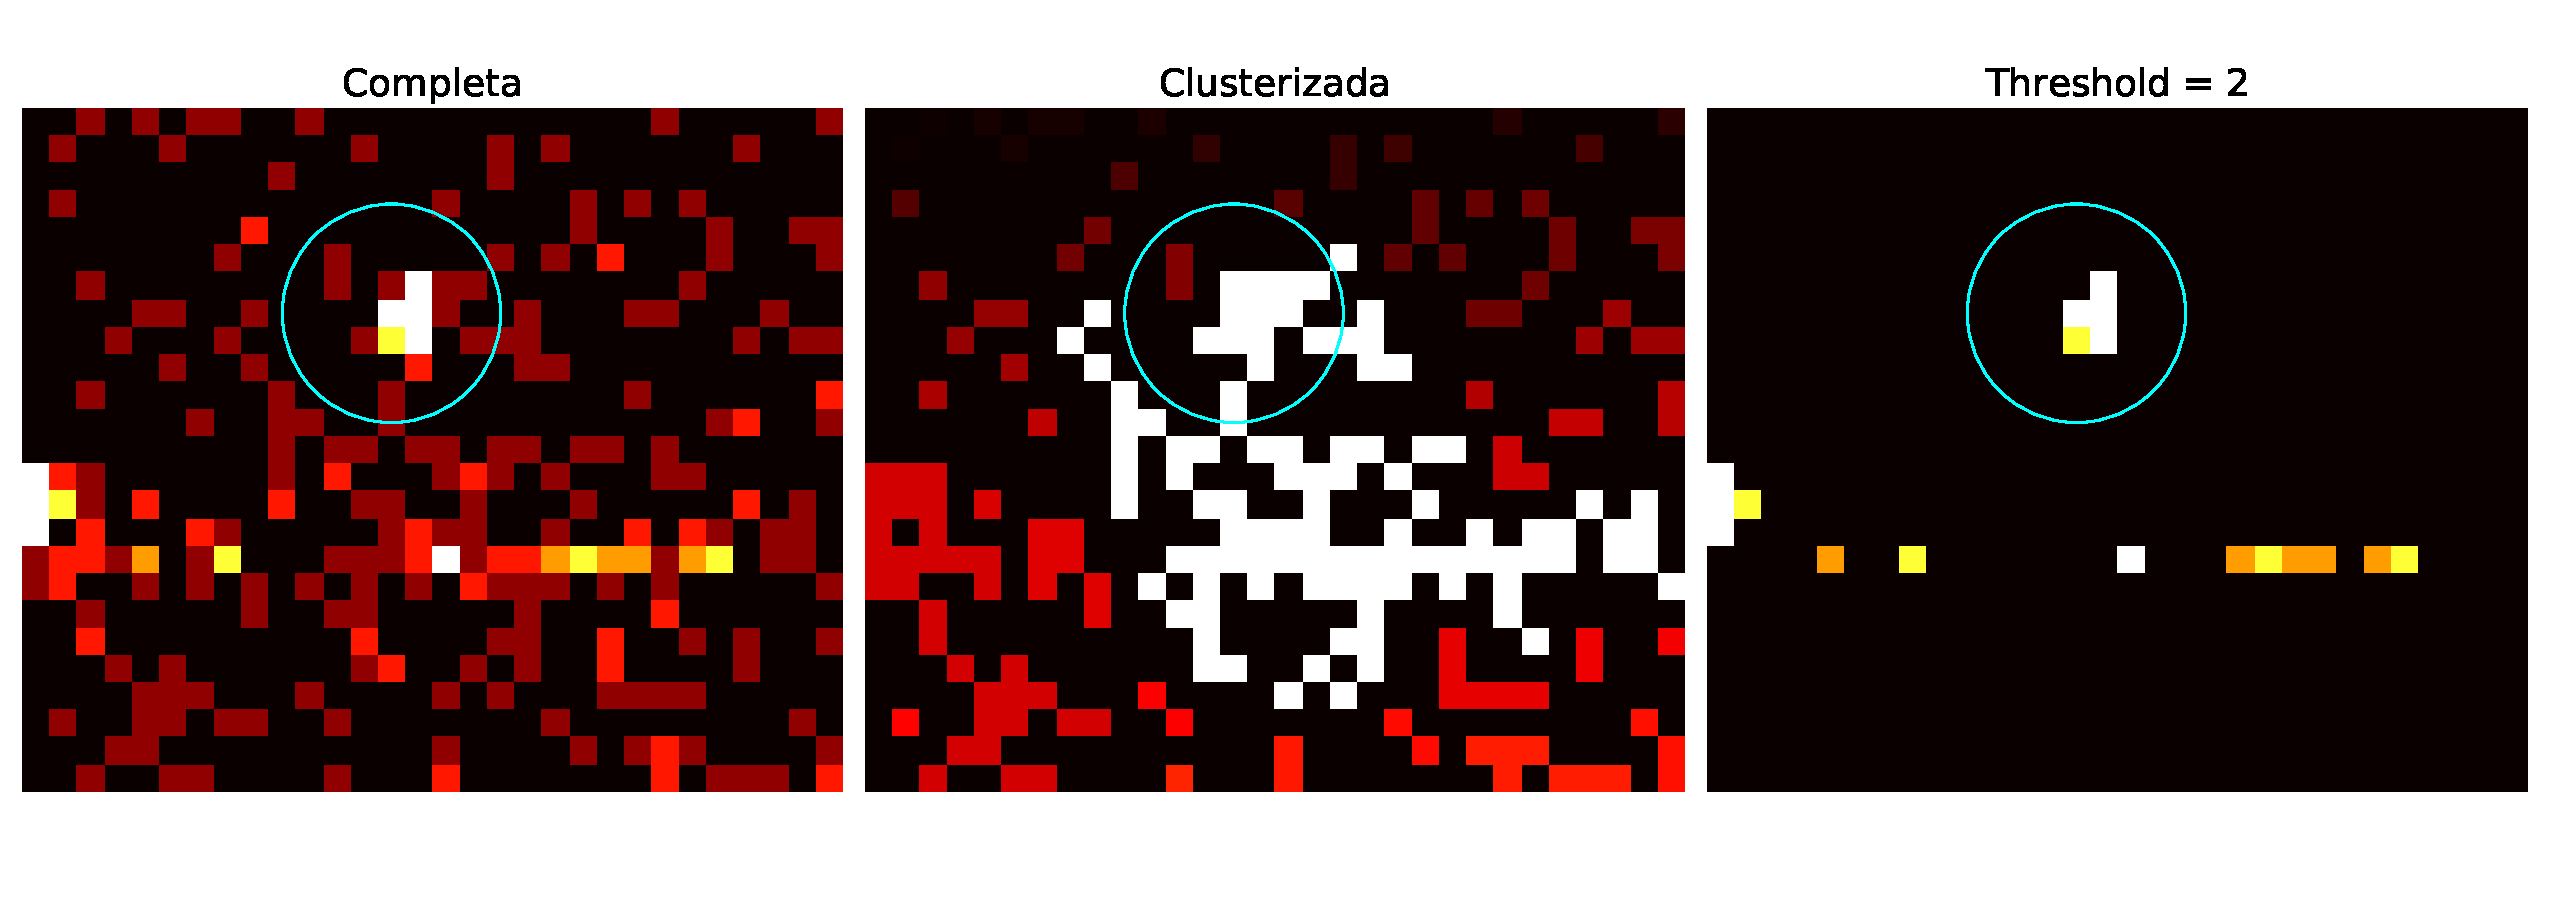
\includegraphics[scale=0.4]{Figs/despegoteo_clusters.pdf}
    \caption{\footnotesize{Ejemplo del caso de un de un evento cercano a los $180$ electrones de carga, que son los eventos de interés. En la imagen de la izquierda se ve la imagen completa, es decir, la medición sin alterar (ya convertida a unidades de carga). En la imagen del centro se en blanco y en un degrade muy tenue de rojos los diferentes clusters que el algoritmo logra reconocer. Lo importante de esta imagen es notar que el algoritmo reconoce como un unico cluster (blanco) a un número de píxeles muy grande debidido justamente a que píxeles con una unica carga generan la union entre todos ellos. Por último, la imagen de la derecha es contiene el cluster de interes una vez que los eventos de un electrón son desechados del análisis, haciendo que ahora sí se contabilice correctamente el evento de interés. Este es un evento de $174$ electrones de carga.}}
    \label{fig:ClusterPegoteado}
\end{figure}
\textcolor{red}{Acá debería hablar de que igual, al eliminar eventos de hasta 2 electrones, no solo estoy eliminando ruido sino que también estoy seguramente eliminando carga real de los clusters. Y que eso hay que tenerlo en cuenta, pero lo pongo en rojo porque no estoy seguro si lo digo más adelante.}\\
\indent De esta forma, se rehicieron los análisis de las imágenes con diferentes valores del corte de calidad, \verb|EPIX = 1.5|, \verb|EPIX = 2.5| y \verb|EPIX = 3.5| y se compararon los resultados obtenidos, tanto para el conteo total de eventos, como los valores finales del factor de Fano y la energía de creación electrón-hueco. Cabe aclarar que estos son resultados preliminares. Esto se hizo para $3$ de los $4$ cuadrantes del sensor, también llamados OHDU's, y se tuvo en cuenta la suma de los 3 cuadrantes funcionales.\\
\indent En las figuras \ref{fig:EntradasVsEpix}, \ref{fig:FanoVsEpix} y \ref{fig:EnergiadeCreacionVsEpix},  puede verse la variación de estos parámetros dependiendo del valor de umbral usado. El gráfico más importante en este punto es el de la figura \ref{fig:EntradasVsEpix}, donde se ve un drástico aumento en la cantidad de entradas (eventos contabilizados) cuando se varía el \verb|EPIX|. Se graficaron en cada figura las modificaciones para $3$ de los $4$ cuadrantes del sensor y para la suma de los cuadrantes $1$, $3$ y $4$. El cuadrante $2$ no funciona correctamente y por eso sus datos no han sido utilizados.
\begin{figure}[h]
%Para hacer estas figs hay que ir a /home/igna/Escritorio/Tesis2021/Figs/pys_para_plots y correr plots_entries_fano_eh.py que usa los datos que están en /home/igna/Escritorio/Tesis2021/Figs/txts_para_plots y se llaman Entries_count.txt
    \centering
    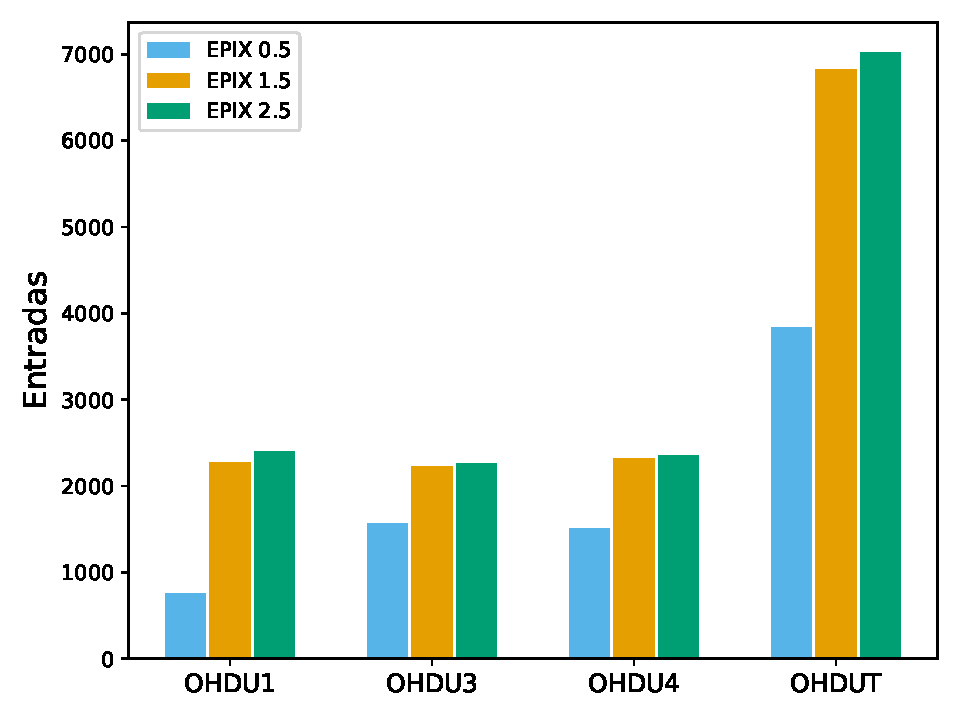
\includegraphics[scale=0.5]{Figs/Entradas_vs_Epix.pdf}
    \caption{\footnotesize{asd.}}
    \label{fig:EntradasVsEpix}
\end{figure}
Se puede ver como los cuadrantes $1$, $3$ y $4$ tienen un cambio pronunciado en la cantidad de entradas al pasar de \verb|EPIX = 0.5| a \verb|EPIX = 1.5|, lo cual implica un aumento en la estadística, que era lo que se esperaba. En cambio, al pasar de \verb|EPIX = 1.5| a \verb|EPIX = 2.5| el aumento en el número de entradas es mucho menor. Particularmente, el primer cuadrante tiene un aumento muy importante en la cantidad de entradas en relación a los otros cuadrantes. Si bien el aumento sigue siendo pronunciado, para los cuadrantes $3$ y $4$ el aumento es menor. En la tabla \ref{tab:EntriesVsEpix} están los valores precisos del cambio en el número de entradas para cada cuadrante para cada valor de \verb|EPIX|. El primer cuadrante pasa de tener $760$ entradas para \verb|EPIX = 0.5| a tener $2272$ para un \verb|EPIX = 1.5|, casi el triple, es un aumento de $\sim 198\%$. En cambio, los cuadrantes $3$ y $4$ pasan de tener $1571$ y $1503$ entradas a $2229$ y $2320$, un aumento muy similar y en torno al $\sim40\%$ y $\sim50\%$ respectivamente.
\begin{table}[]
\centering
\begin{tabular}{@{}c|c|c|c|c@{}}
\toprule
           & OHUD 1 & OHDU 3 & OHDU 4 & OHDU 1 + 3 + 4 \\ \midrule\hline
EPIX = 0.5 & 760    & 1571   & 1503   & 3834           \\
EPIX = 1.5 & 2272   & 2229   & 2320   & 6821           \\
EPIX = 2.5 & 2399   & 2261   & 2356   & 7016           \\ \bottomrule
\end{tabular}
\caption{tabla}
\label{tab:EntriesVsEpix}
\end{table}
Efectivamente se observa un aumento en el conteo de eventos que reconoce el programa al aumentar el valor del parámetro \verb|EPIX|. También se observa que el aumento más pronunciado es desde $0.5$ a $1.5$. El aumento promedio en el conteo de eventos es de alrededor del $100\%$.
\begin{figure}[h]
%Para hacer estas figs hay que ir a /home/igna/Escritorio/Tesis2021/Figs/pys_para_plots y correr plots_entries_fano_eh.py que usa los datos que están en /home/igna/Escritorio/Tesis2021/Figs/txts_para_plots y se llaman Entries_count.txt
    \centering
    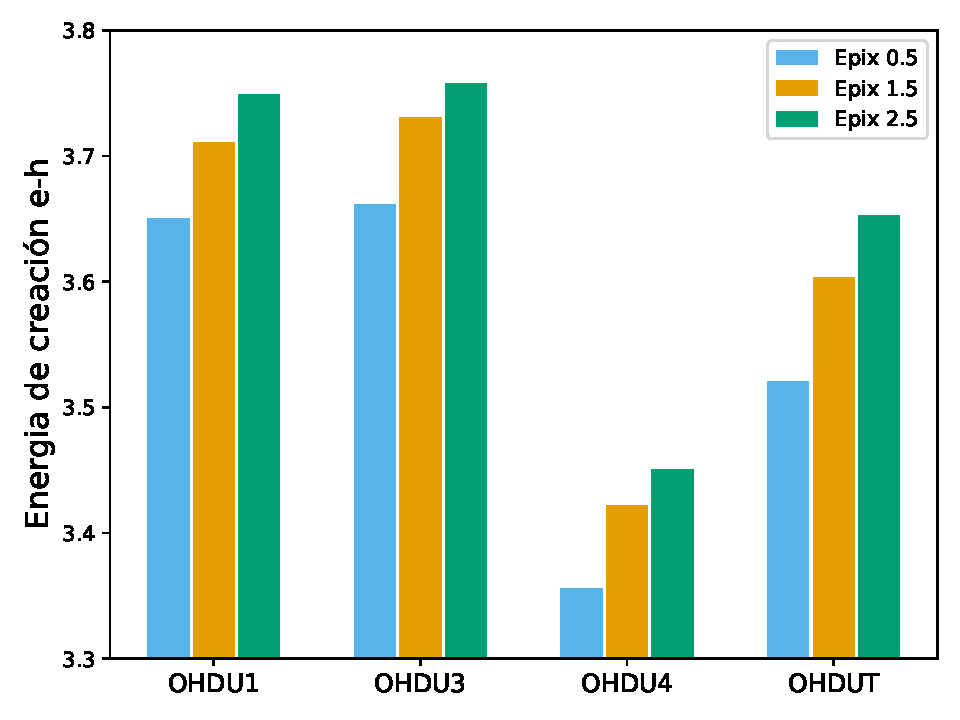
\includegraphics[scale=0.5]{Figs/EnergiaCreacion_vs_Epix.pdf}
    \caption{\footnotesize{asd.}}
    \label{fig:EnergiadeCreacionVsEpix}
\end{figure}
En cuanto al gráfico de la figura \ref{fig:EnergiadeCreacionVsEpix}, se ve como el valor preliminar para la energía de creación electrón hueco aumenta en todos los casos al aumentar el umbral \verb|EPIX|. Esto puede deberse al efecto que genera aplicar un umbral y disminuir la carga en los clusters contabilizados, que a su vez son más. Puede suceder que la cantidad de carga en los clusters sufra un corrimiento a la izquierda del valor medio real y por esto la energía de creación electrón-hueco aumente al aumentar el \verb|EPIX|: A un mismo valor de energía, una menor carga ionizada implica una mayor energía de creación electrón-hueco.
Finalmente, el caso más irregular corresponde al gráfico de la figura \ref{fig:FanoVsEpix}, donde cada cuadrante y para cada valor de \verb|EPIX| el factor de Fano dio valores diferentes y no puede definirse una tendencia a partir de estos resultados.
\begin{figure}[h]
%Para hacer estas figs hay que ir a /home/igna/Escritorio/Tesis2021/Figs/pys_para_plots y correr plots_entries_fano_eh.py que usa los datos que están en /home/igna/Escritorio/Tesis2021/Figs/txts_para_plots y se llaman Entries_count.txt
    \centering
    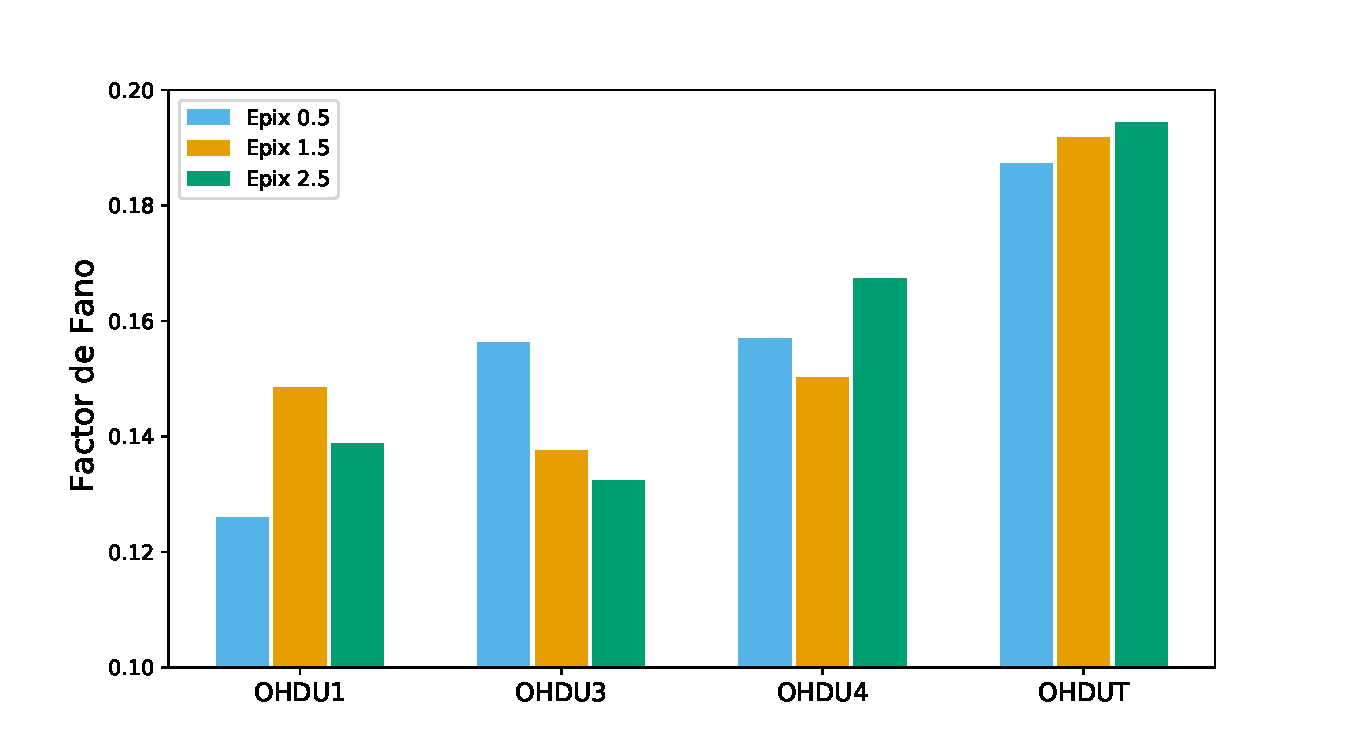
\includegraphics[scale=0.5]{Figs/Fano_vs_Epix.pdf}
    \caption{\footnotesize{asd.}}
    \label{fig:FanoVsEpix}
\end{figure}
Entonces, del análisis preliminar modificando el umbral conteo de carga por píxel se puede observar el aumento deseado en la estadística para los eventos de interés de este trabajo. Como se observa que el mayor aumento en la estadística se da para \verb|EPIX = 1.5|, ese es el valor de umbral con el que se realizan los subsiguientes análisis. No está de más recordar que ese valor de umbral implica desechar los píxeles que tengan $2$ o menos electrones de carga.\\
\indent 
\indent Entonces, con este resultado se plantea buscar las correcciones necesarias a ser aplicadas, debido a la eliminación de carga que genera el umbral usado para aumentar la estadística. En adelante, la idea es intentar compromender el ruido de fondo en las imágenes y con ello poder corregir los valores de carga de los clústeres.

%%%%%%%%%%%%%%%%%%%%%%%%%%%%%%%%%%%%%%%%%%%%%%%%%%%%%%%%%%%%%%%%%%

\chapter{Imágenes y análisis}
\section{Preliminares}
El análisis realizado al variar el \verb|EPIX| se llevó a cabo sin la necesidad de \textit{observar} las imágenes de las cuales se extraen los datos. %Los análisis realizados modificando el \verb|EPIX| para aumentar la estadística de los datos se realizaron sin la necesidad de observar cada una de las imágenes.
Sin embargo, conocer los datos y poder identificar características de las imágenes es un factor sumamente importante para comprender los resultados. Con este fin, se hizo un análisis visual, cualitativo y cuantitativo de las imágenes para comprender mejor los datos, explorar las características del sensor y de cada uno de sos cuadrantes y poder reconocer posibles deficiencias.\\
\indent Uno de los primeros factores a caracterizar es el ruido en el sensor, donde por ruido se entiende a todos aquellos píxeles con una única carga (un electrón) que no es debida eventos de ionización. El ruido puede ser producto de corrientes oscuras (electrones excitados espontáneamente que dejar con carga un píxel), rebotes de un haz de baja energía en la cámara donde se encuentra el sensor y producen eventos que no son de interés en un determinado píxel, etc. Una forma de caracterizarlo es tomar las imágenes y extraer todos los píxeles donde la carga sea mayor que un electrón. De este modo, se obtienen imágenes donde solo hay eventos de un electrón y así son fácil de caracterizar. Por ejemplo, se pueden sumar todas y promediarlas, de esta forma se puede ver si existen regiones con mayor o menor tendencia a concentrar este tipo de eventos.\\
\indent En la figura \ref{fig:Eventos1e} se tiene una imagen por cada cuadrante del sensor, promediados en las $925$ imágenes tomadas, donde los píxeles más brillantes son los son los que tienen mayor promedio de eventos. Puede interpretarse como una imagen de la probabilidad por píxel de que haya un único electrón. Entre las características que más se destacan de estas imágenes, se encuentran:
\begin{itemize}
    \item La ausencia de carga (en promedio) en las regiones del pre-scan (región izquierda de 8 columnas de píxeles de extensión) y del over-scan (región derecha de 50 columnas de píxeles de extensión) lo cual es totalmente esperable.
    \item El primer cuadrante es en promedio más brillante que el resto, y se observa un ligero gradiente de color entre las filas inferiores y superiores. Esto se repite, pero en menor medida en los demás cuadrantes.
    \item El segundo cuadrante (OHDU 2) capta en promedio muy poca carga. Este cuadrante del sensor es defectuoso.
    \item En los cuadrantes $3$ y $4$ se pueden ver columnas enteras de píxeles oscurecidas, que captaron muchísima menos carga (defectos del sensor?).
    \item En todos los cuadrantes (menos el segundo), se observa un único píxel (posición $x = 2$, $y = 0$) donde el promedio de carga es mucho mayor al resto. Además, la primera columna de píxeles luego del pre-scan también tiene tendencia a captar más carga que el resto.
\end{itemize}

\begin{figure}[H]
%Para reproducir esta figura hay que ir al directorio /home/igna/Escritorio/Tesis2021/Figs/pys_para_plots y correr skipper_cuadrantes_plot.py
    \centering
    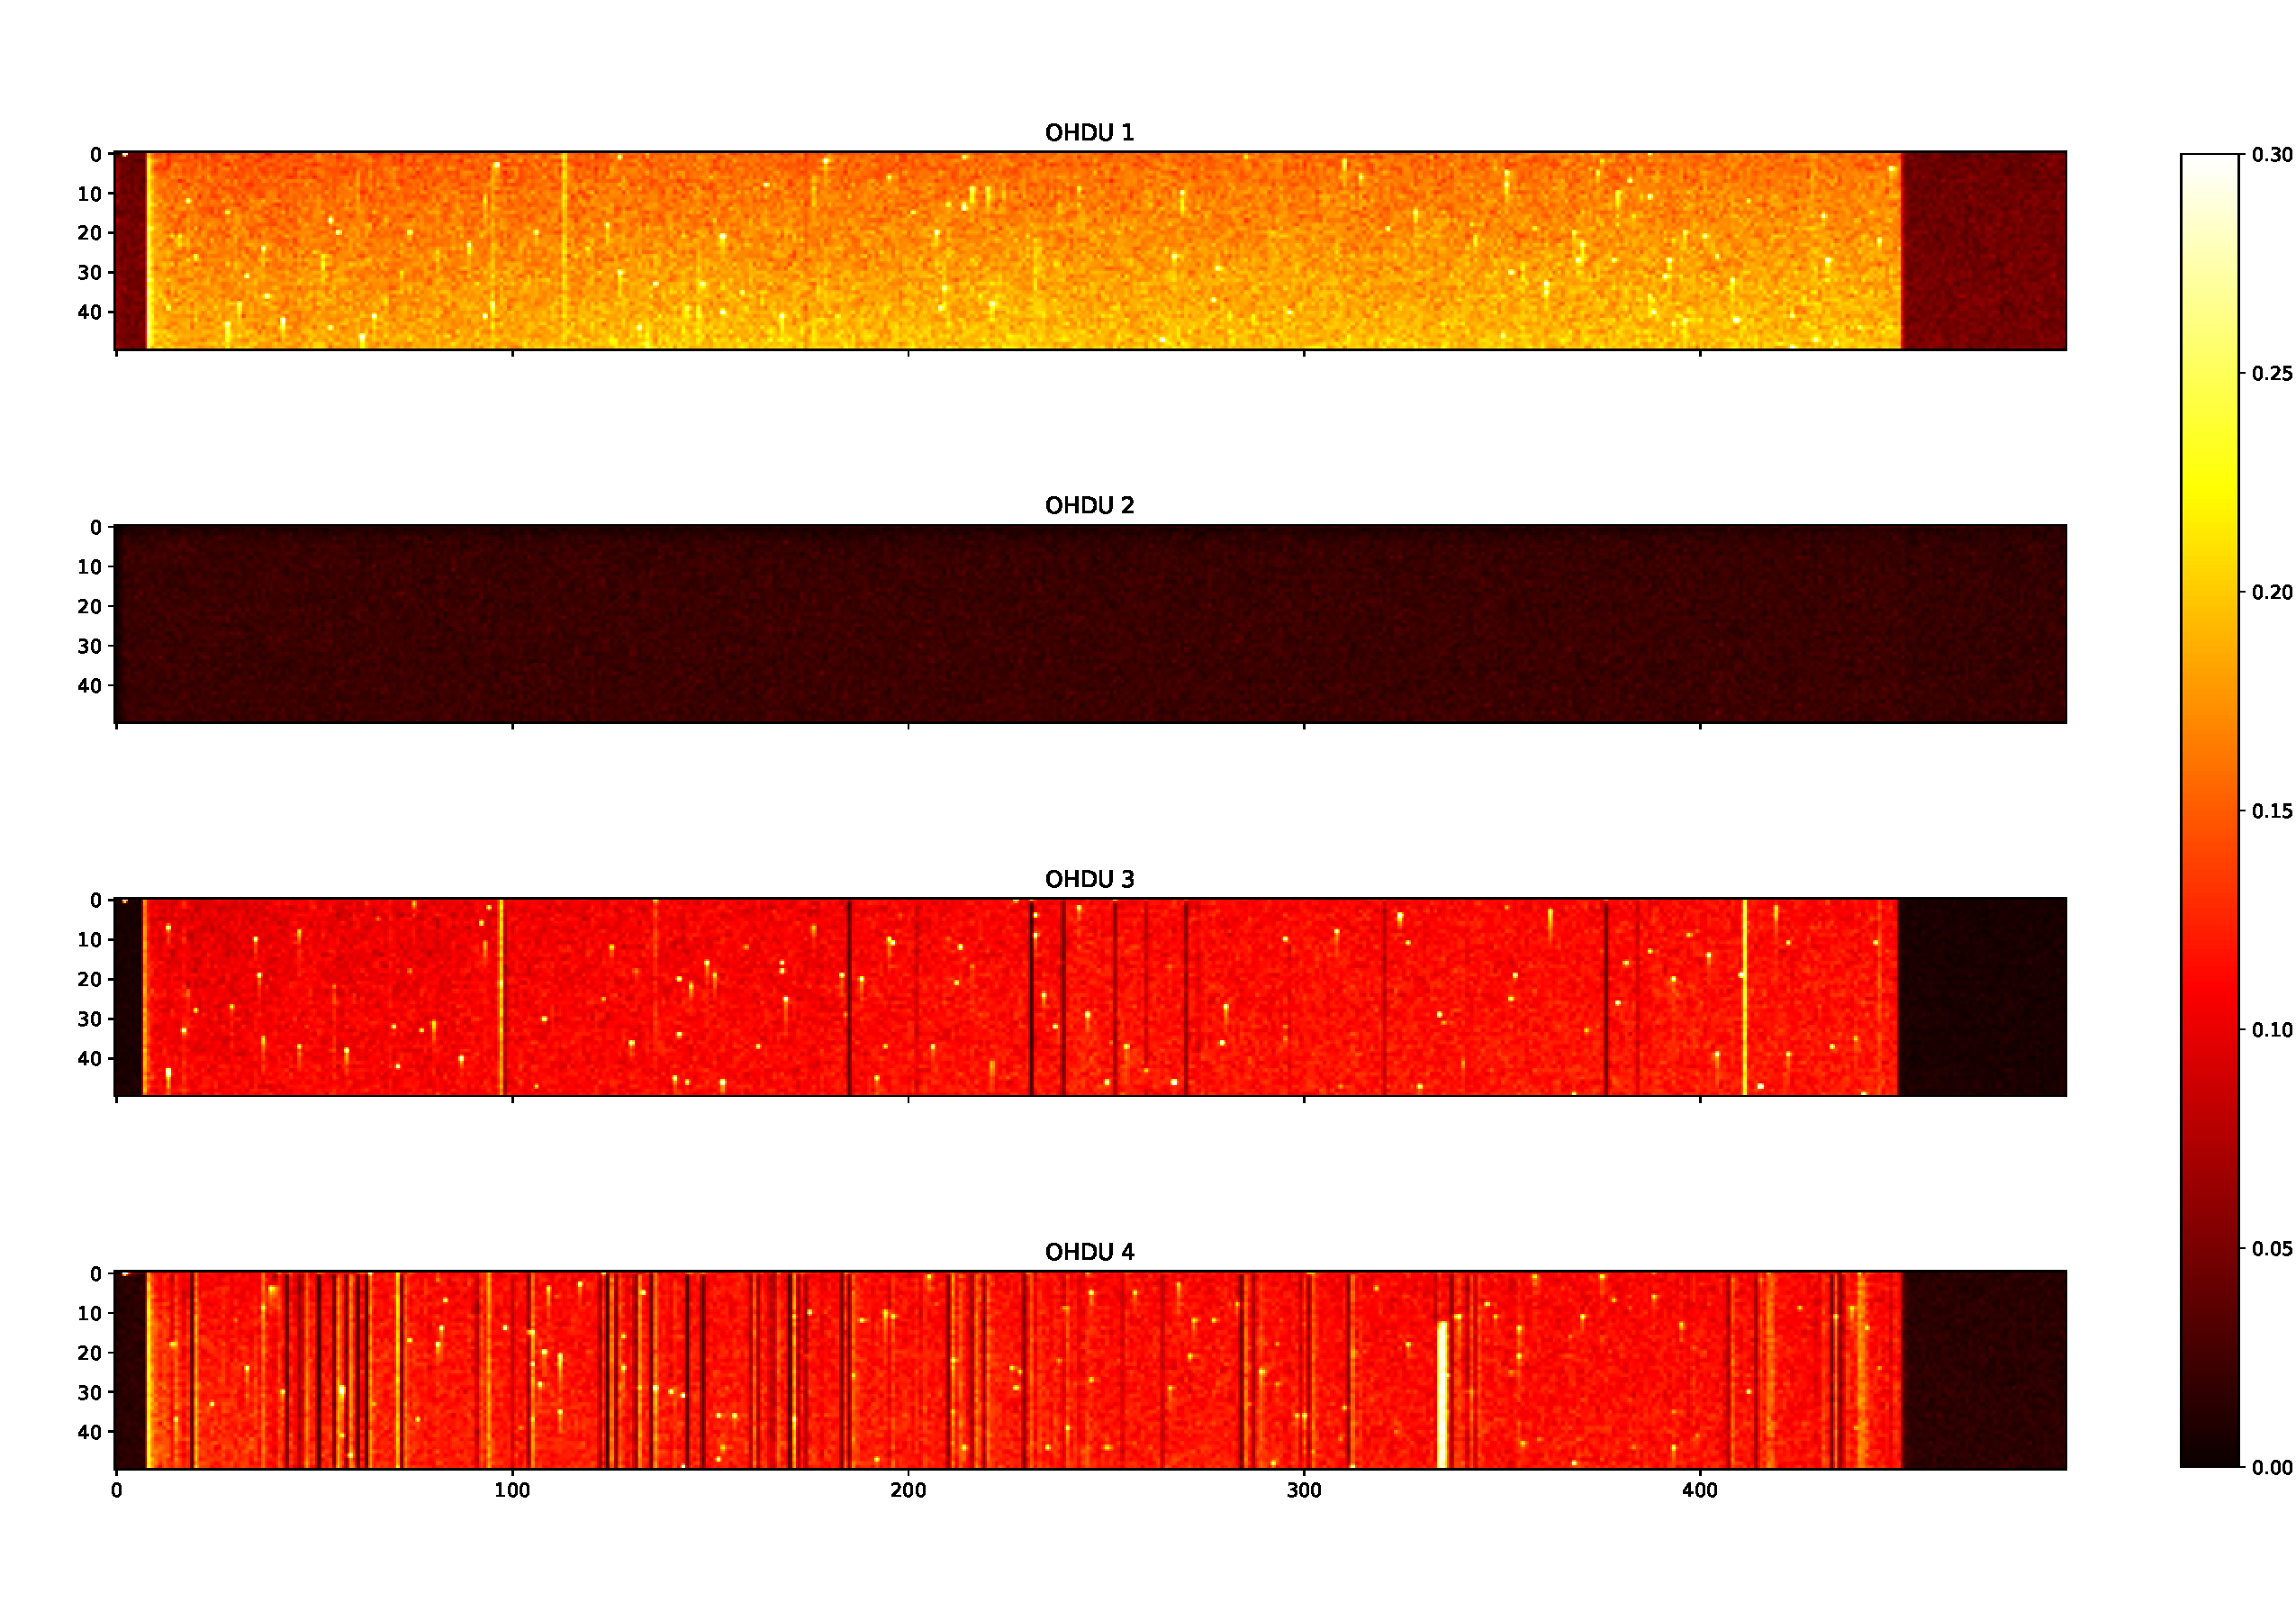
\includegraphics[scale=0.4]{Figs/1ePromedio.pdf}
    \caption{\footnotesize{asd.}}
    \label{fig:Eventos1e}
\end{figure}

Respecto al gradiente de color que se observa entre filas superiores e inferiores, puede interpretarse como una mayor probabilidad de que en promedio los píxeles de las filas inferiores tengan una carga mayor que en las filas superiores. Esto puede observarse en los gráficos de figura \ref{fig:GradienteProb}, donde se ve el aumento en \textit{la probabilidad} media por fila de que haya un evento de un electrón, a medida que el número de la fila aumenta. Esto puede deberse a que las filas superiores del sensor son las primeras a las que se les mide la carga, generando que las filas inferiores permanezcan más tiempo expuestas a fuentes de eventos. De todas maneras esta diferencia de tiempo en la lectura de las diferentes filas del sensor es muy pequeña
\begin{figure}[H]
%Para modificar este plot hay que ir a /home/igna/Escritorio/Tesis2021/Figs/pys_para_plots y correr gradiente_filas_sensor.py Los datos los saca de /home/igna/Escritorio/Tesis2021/Figs/txts_para_plots y del archivo OHDU1/2/3/4_gradiente_filas_sensor.tx
    \centering
    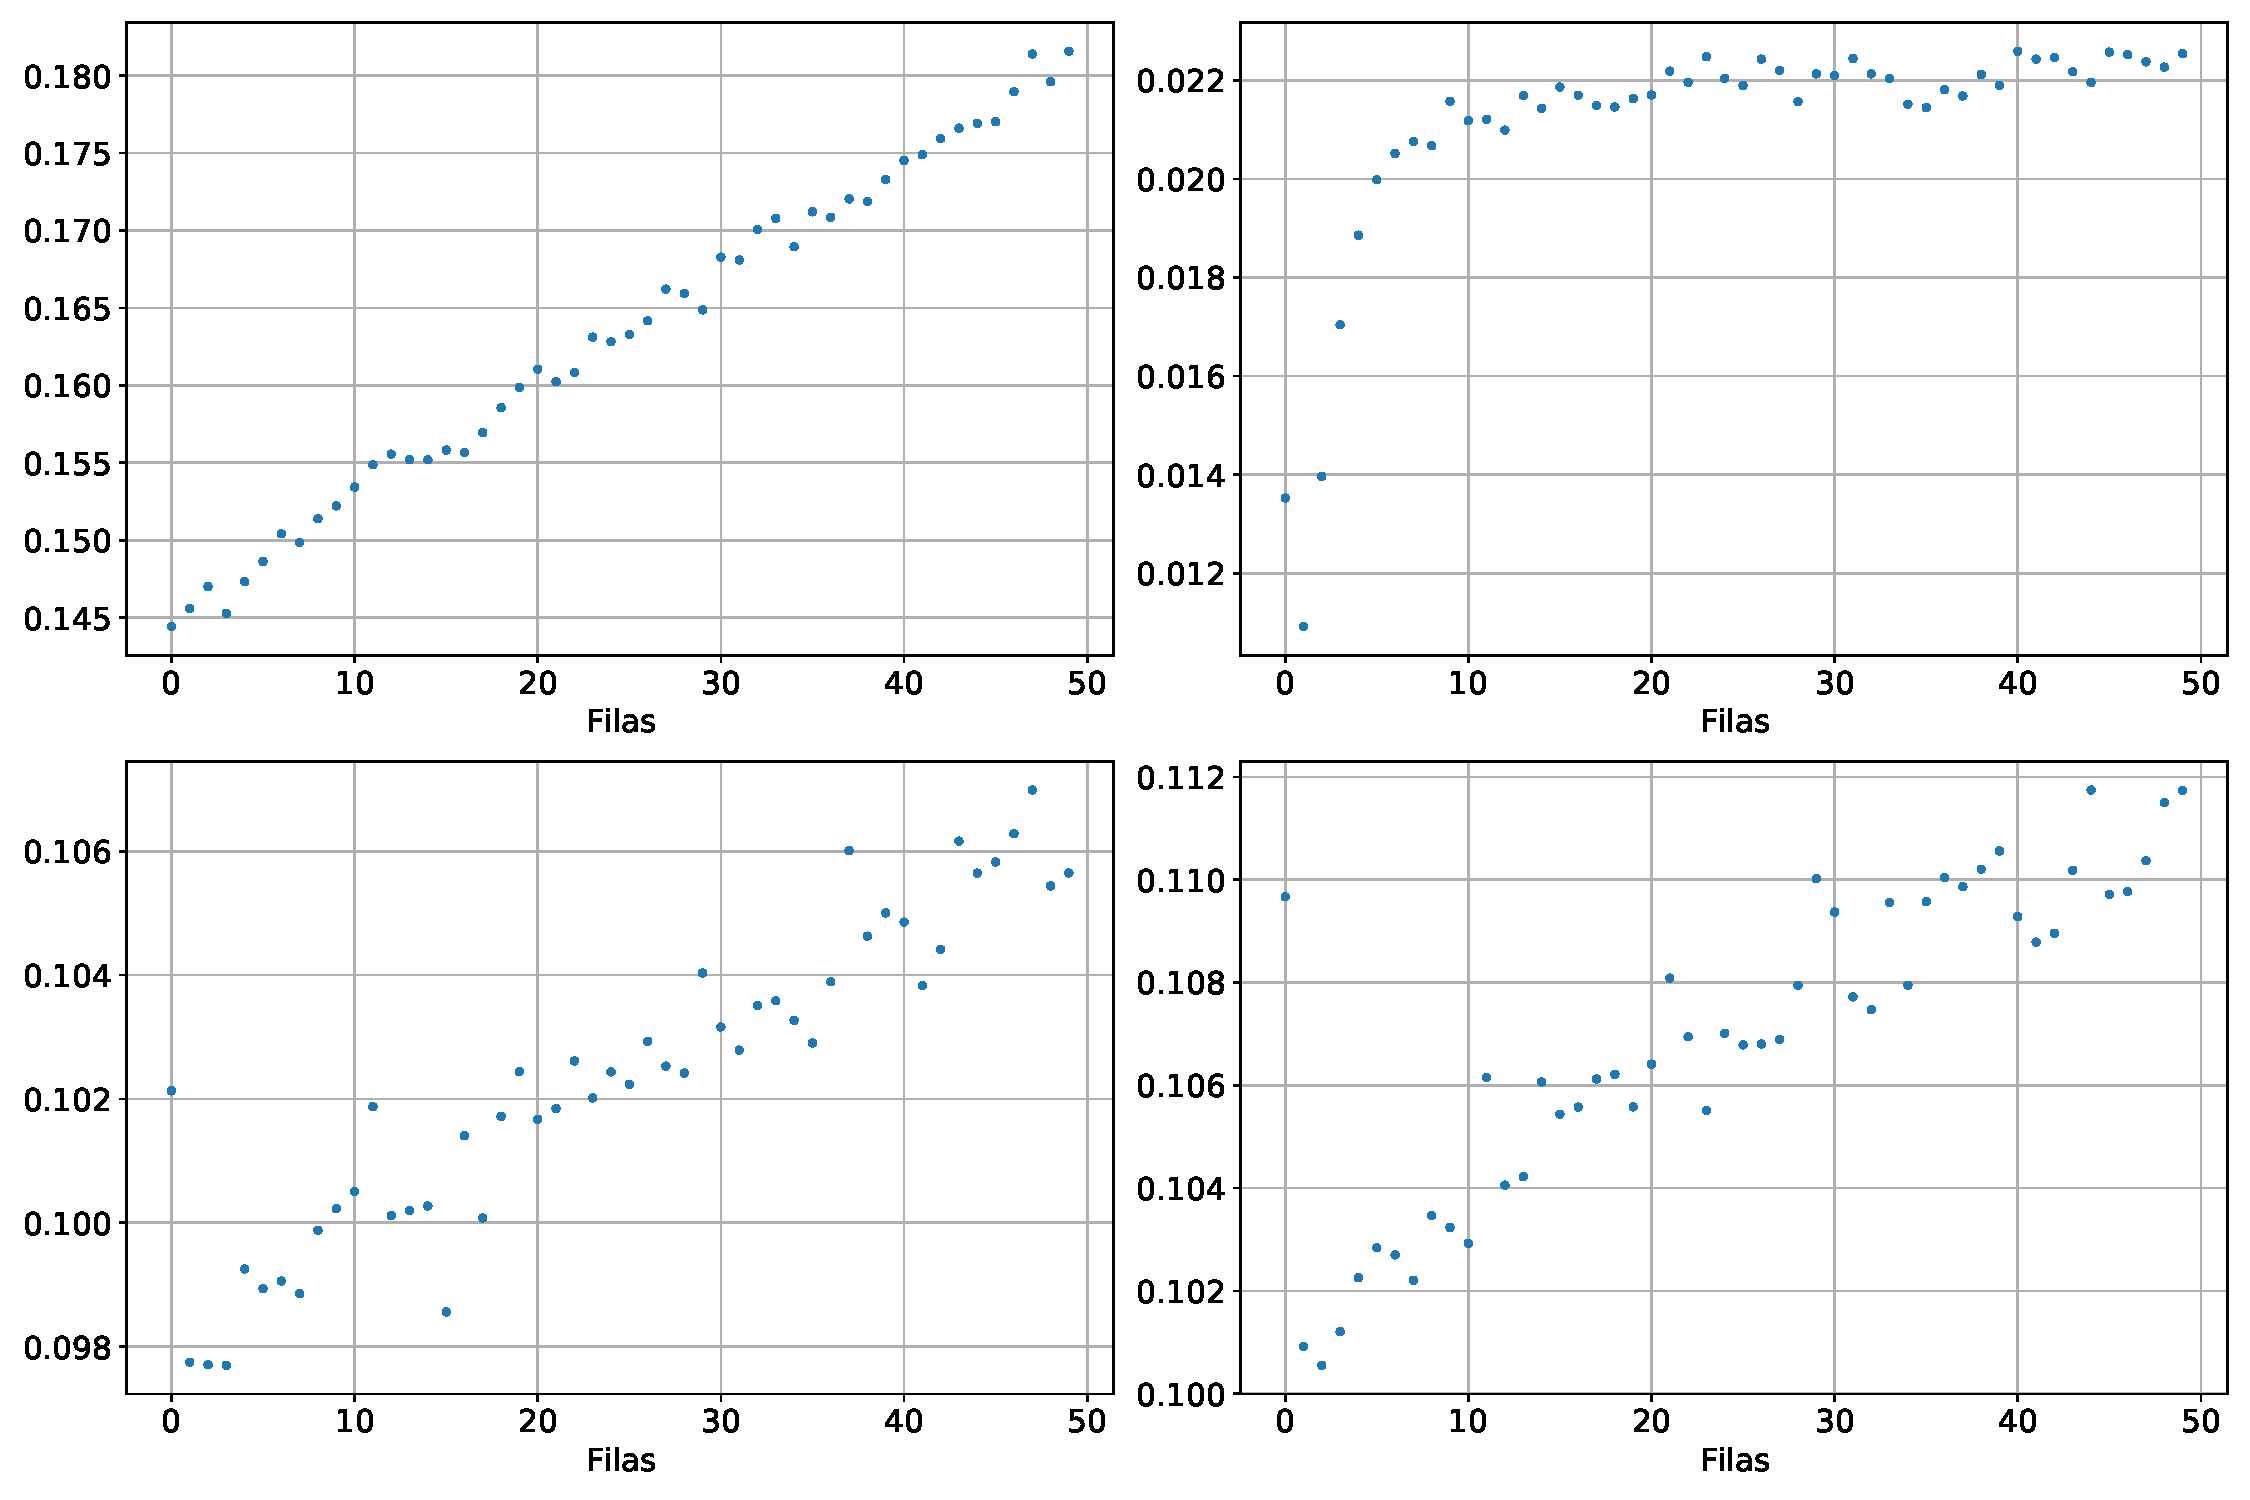
\includegraphics[scale=0.45]{Figs/Gradiente_en_filas_sensor.pdf}
    \caption{\footnotesize{asd.}}
    \label{fig:GradienteProb}
\end{figure}
Todos los análisis subsiguientes fueron realizados principalmente con el primer cuadrante del sensor, dado que es el cuadrante que funciona mejor.\\
\indent En la búsqueda por caracterizar el ruido en el sensor, lo que se hizo fue promediar la imagen resultante del promedio de las $925$ imágenes, de forma de obtener una \textit{probabilidad} general de que en un píxel haya un evento de un electrón. De hacer esto, para el primer cuadrante y considerando solo la región activa del sensor, se obtuvo una probabilidad $p = 0.1762 \pm 0.021$.\\
\indent Sin embargo, esta forma de caracterizar el ruido en el sensor es muy burda y no es correcta. Un camino un poco más sofisticado para estimar el ruido en el sensor es explotando el hecho de que los eventos medidos en él siguen una distribución Poissoniana, de forma que si se pudiera calcular la esperanza $\mu$ de la distribución, podría saberse la probabilidad de que en un determinado píxel se encuentre un evento de un electrón.\\

\section{Estimación de la esperanza de la distribución}
\noindent Si se considera una distribución Poissoniana para la variable aleatoria \textit{número de electrones por píxel}, se puede tomar el caso $p = P(k = 1 | \mu) = 0.1762 \pm 0.0210$, que es la probabilidad que se obtuvo previamente. De forma iterativa, se halla el valor de la esperanza de la distribución: $\mu = 0.2194 \pm 0.0001$.\\
\indent Otra forma de calcular la esperanza de la distribución es notando lo siguiente: Si se toman las probabilidades de que haya una sola carga por píxel y que no haya ninguna carga por pixel, es decir
\begin{equation*}
    p_{0} \equiv P(k = 0 | \mu),
    \quad
    \quad
    p_{1} \equiv P(k = 1 | \mu)
\end{equation*}
y se mira la relación entre ambas, se tiene
\begin{equation*}
    \frac{p_{1}}{p_{0}} = \frac{\mu\,e^{-\mu}}{e^{-\mu}} = \mu
\end{equation*}
y se ve que puede hallarse directamente el valor de la esperanza de la distribución. Traducir esto sobre las imágenes no es más que contar la cantidad de píxeles con una única carga y los píxeles sin ninguna carga y ver la relación entre ambas. De esto se obtuvo que el valor de la esperanza es 
\begin{equation*}
    \mu = 0.2245 \pm 0.0001
\end{equation*}
Si bien esta forma de estimar la esperanza de la distribución es un poco más sofisticada que la anterior, todavía no se están teniendo en cuenta algunos factores que podrían añadir sesgo.\\
\indent No hay que perder de vista que la utilidad de calcular la esperanza de la distribución es poder utilizarla luego para estimar cuánta carga sobre los clústers es debida a ruido. Conociendo la esperanza de la distribución del ruido y la cantidad de píxeles que ocupa un clúster, puede calcularse la cantidad esperada de carga extra debido a ruido que se halla en cada clúster. Teniendo estos valores, puede corregirse entonces el valor de la carga y con eso hacer mejores estimaciones del factor de Fano y la energía de creación electrón-hueco.\\
\indent Pero también, para poder generar una corrección en el conteo de cargas por cluster y que esté lo menos sesgada posible, hay que tener en cuenta las posibles formas en las que un clúster podría tener más o menos carga. Podría suceder que sobre la superficie de los clústers hayan eventos de más, debido a corrientes oscuras u cualquier forma de ruido del sensor. Pero también, dado que en este análisis se está aplicando un corte de calidad que elimina eventos de $1$ electrón, podría suceder que a un clúster se le quiten eventos reales que se encuentran en sus bordes. Con lo cual no solo es necesario corregir la carga por exceso en los clusters, sino también por defecto.\\
\indent La esperanza que se obtuvo de calcular la relación entre eventos de $1$ electrón y píxeles vacíos contiene entonces, tanto información de eventos espúrios como información de eventos genuinos. Pero lo que se persigue es poder identificar los eventos de ruido y los genuinos por separado. En ese sentido puede decirse que 
\begin{equation*}
    \mu_{T} = \mu_{bkg} + \mu_{g}
\end{equation*}
donde $\mu_{bkg}$ es la esperanza de la distribución de la variable aleatoria \textit{cantidad de eventos espurios por píxel}, mientras que $\mu_{g}$ es la esperanza de la variable aleatoria \textit{cantidad de eventos genuinos por píxel}. Hay que lograr separar ambos efectos para poder aplicar las correcciones correctamente.

\subsection{Análisis de los bordes de los clústers}
La forma en la que se buscó poder separar ambas contribuciones al calcular el $\mu_{T}$ de la distribución fue mirando los bordes de los clusters y no todo el sensor. Ahora, en vez de tomar la imagen que tiene solo eventos de $1$ electrón, se toma la imagen que tiene los eventos de $2$ o más electrones y con ella se genera una máscara de los bordes de estos. Como la idea es corregir la carga en los clústers, tiene sentido mirar en el entorno de estos y no en todo el sensor.\\
\indent El procedimiento consiste en tomar los clústers y hacer una máscara de su contorno, expandiéndola en un píxel en todas las direcciones. Luego, superponiendo la máscara sobre la imagen original (con todos los eventos), se cuenta cuántos eventos cayeron dentro de la máscara. Nuevamente, haciendo la relación entre eventos de un electrón y píxeles vacíos, se calcula el $\mu_{T}$. Se estima que en el borde inmediato a los clústers existe contribución de ambos efectos: eventos espurios y eventos genuinos. Por otro lado, para calcular la contribución de los eventos espurios, se hace el mismo procedimiento pero expandiendo los clústers en dos pixeles en todas las direcciones, y quedándose únicamente con el segundo borde, donde claramente no puede haber contribución de eventos genuinos de un cluster. Nuevamente, de la relación entre los eventos de $1$ electrón y los píxeles vacíos, se obtiene $\mu_{bkg}$ y con este, puede despejarse el valor $\mu_{g}$.\\
\indent La razón por la cual se usan los eventos inmediatamente contiguos a los bordes de los clusters para calcular el $\mu_{T}$, es porque se puede decir con seguridad que es la única región del sensor donde coexisten ambas contribuciones: $\mu_{bkg}$ y $\mu_{g}$. Tanto los eventos de un electrón que realmente pertenecen a los clusters como los eventos de un electrón que son espurios. Por otro lado, la razón por la cual se estima $\mu_{bkg}$ del siguiente cordón ($2$ píxeles de distancia al borde del clúster) se debe a que en esa zona es seguro que no pueden haber eventos genuinos de un clúster (o al menos la probabilidad de que eso suceda ronda los $10\times 10^{-14}$).\\
\indent El valor de la esperanza de ambas contribuciones resultó $\mu_{T} = 0.19735 \pm 0.00024$ yel valor de la esperanza para los eventos espurios resultó $\mu_{bkg} = 0.18583 \pm 0.00021$, con lo cual, la esperanza para los eventos genuinos es $\mu_{g} = 0.011524 \pm 0.00003$. Teniendo estos valores puede corregirse el conteo de carga en los clústeres, tanto por exceso como por defecto y así tener una medición más precisa del factor de Fano y la energía de creación electrón-hueco.

\subsection{Corrección del conteo de carga}
\noindent La corrección del conteo de carga se llevó a cabo modificando el código del programa que con root calcula el factor de Fano, la energía de creación electrón-hueco, y otras variables, por medio del ajuste de los histogramas de carga. El programa se encarga de procesar todas las imagenes, desechar eventos que tengan carga menor a $2$ electrones (\verb|EPIX = 1.5|), buscar los clusters, quedarse únicamente con aquellos que tengan cargas en el entorno de los $180$ electrones y calcular esos valores. Al contar la carga de estos clusters, se agrega y se quita carga en función los valores hallados antes.\\
\indent Dado que la distribución de la variable aleatoria \textit{cantidad de eventos por píxel} sigue una distribución poissoniana de esperanza $\mu$, para cada tipo evento (espurio, genuino o total) se tiene una esperanza. Para calcular la cantidad de carga que se espera que tenga un cluster de $N$ píxeles en el sensor, se puede hacer uso de las propiedades de la esperanza. Sea $Y = \sum\limits_{i = 1}^{N} X_{i}$, donde $X_{i}$ son distintas realizaciones de la variable aleatoria con distribución Poissoniana y $N$ es el número de píxeles del cluster, entonces la esperanza se calcula como
\begin{equation*}
    E(Y) = 
    E
    \left(
        \sum\limits_{i=1}^{N} X_{i}
    \right)
    = \sum\limits_{i=1}^{N}E(X_{i})
    = \sum\limits_{i=1}^{N}\mu_{i}
\end{equation*}
pero como $X_{i}$ son distintas realizaciones de la misma variable aleatoria, entonces tiene todas la misma esperanza, es decir $\mu_{i} = \mu\ \forall\ i$, con lo cual
\begin{equation*}
    E(Y) = N\mu
\end{equation*}
con lo cual, la cantidad de carga esperada para un cluster viene dada por la esperanza de la distribución, por la cantidad de píxeles. De esta forma, teniendo una esperanza total $\mu_{T} = \mu_{bgk} + \mu_{g}$, aplicando esta misma receta pueden corregirse los valores de carga por cluster. Sea $n_{e}$ la cantidad de carga medida en un dado cluster, la corrección de este valor de carga será $n_{c}$ y viene dado por
\begin{equation*}
    n_{c} = n_{e} + N\mu_{g} - N\mu_{bkg}
\end{equation*}
es decir, se agrega la cantidad de carga genuina que se estima se pierde por aplicar \verb|EPIX = 1.5| y se quita la carga estimada por ruido. \textcolor{red}{Acá no me queda del todo claro como era el tema del redondeo: $N\mu_{g}$ y $N\mu_{bkg}$ claramente son float, pero la carga tiene que ser entera. El redondeo donde se hacía?}


\newpage
Acá va a ir el análisis y manejo de las imágenes, con las diferentes pruebas que se fueron haciendo, primero para entender los datos con los que se está tratando (hablar de dónde el sensor es más propenso a ver ruido, por qué siempre hay un pixel brillante, por qué hay lineas verticales brillantes, por qué hay cuadrantes con tanto ruido, cuadrantes que andan mal, qué cuadrante usé, por qué?).\\
\indent Luego los diferentes approaches que se hicieron para tratar de estimar el ruido por background que mete un bias en el conteo de carga de los eventos de interés:
\begin{itemize}
    \item Primero lo que hice fue agarrar la imagen y quedarme solo con los eventos de 1 electrón, transformando a 0 la carga en los demás píxeles y promediando en todas las imágenes esta cantidad y así obtener una probabilidad de que en un dado píxel halla un electrón de ruido. Explicar por qué este approach no es del todo correcto 
    \item Segundo, manteniendo este approach, usarlo para estimar el $\mu$ de la distribución poissoniana de la variable aleatoria "cantidad de carga por píxel"
    \item Tercero, estimar el ruido pero sólo mirando en los contornos de los clusters, debido a que en estas regiones es donde se elimina carga al usar el epix=1.5 y porque encima de los clusters es donde se agrega carga espuria por ruido.
\end{itemize}
Una vez explicados los approachs que usé y por qué se fueron refinando, hablar de la corrección final a aplicar y como se aplica en el software ya armado para el cálculo del factor de fano y de la energía de creación electrón hueco.

%%%%%%%%%%%%%%%%%%%%%%%%%%%%%%%%%%%%%%%%%%%%%%%%%%%%%%%%%%%%%%%%%%

\chapter{Resultados}
Sección pendiente porque faltan los resultados.

%%%%%%%%%%%%%%%%%%%%%%%%%%%%%%%%%%%%%%%%%%%%%%%%%%%%%%%%%%%%%%%%%%

\chapter{Conclusiones}
faltan las conclusiones